%************************************************
\chapter{The Planning Machine}
\label{chapter:the_planning_machine}
%************************************************



\section{Plan Operators}

In the implementation, plans are composed of four basic types of plan
operators.
\begin{enumerate}
\item The \emph{resource activation operator} references a
  counterfactual transframe, which includes specific resource
  activation dependencies as well as specific hypothesis dependencies.
\item The \emph{resource suppression operator} references a resource
  that should be suppressed when this operator is executed.
\item The \emph{sequential program operator} temporally orders two
  other plan operators.
\item The \emph{parallel program operator} arranges two other plan
  operators to be executed simultaneously.
\end{enumerate}
{\mbox{\autoref{figure:example_plan_operators}}} shows an example of a
plan with four composable plan operators, while
{\mbox{\autoref{figure:example_plan}}} shows a more detailed example
of a two-step plan.
\begin{figure}
\centering
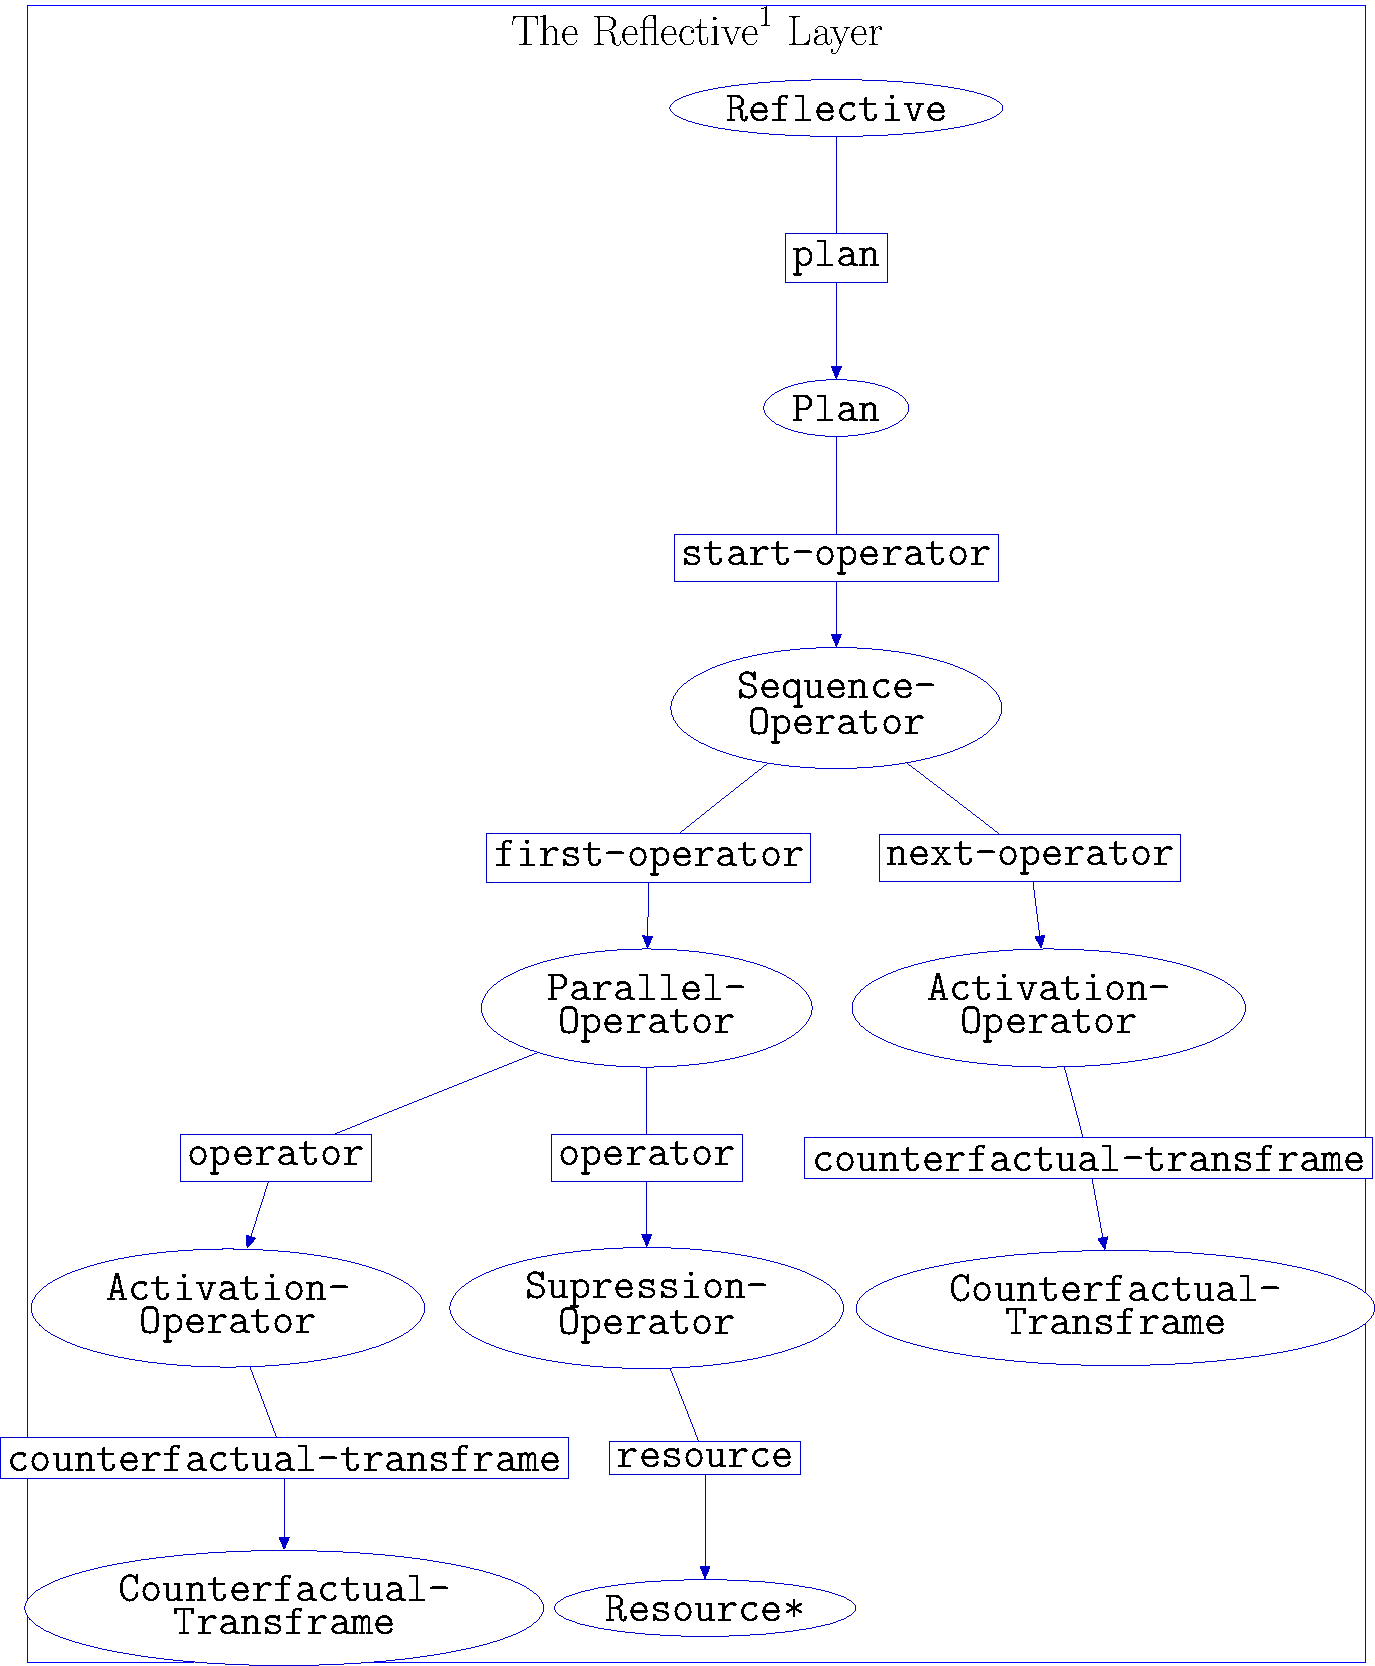
\includegraphics[width=12cm]{gfx/example_plan_operators}
\caption[An example of a plan with four composable plan operators.]{An
  example of a plan with four basic plan operators: (1) the resource
  activation operator, (2) the resource suppression operator, (3) the
  sequential program operator, and (4) the parallel program operator.}
\label{figure:example_plan_operators}
\end{figure}
\begin{figure}
\hspace*{-2cm}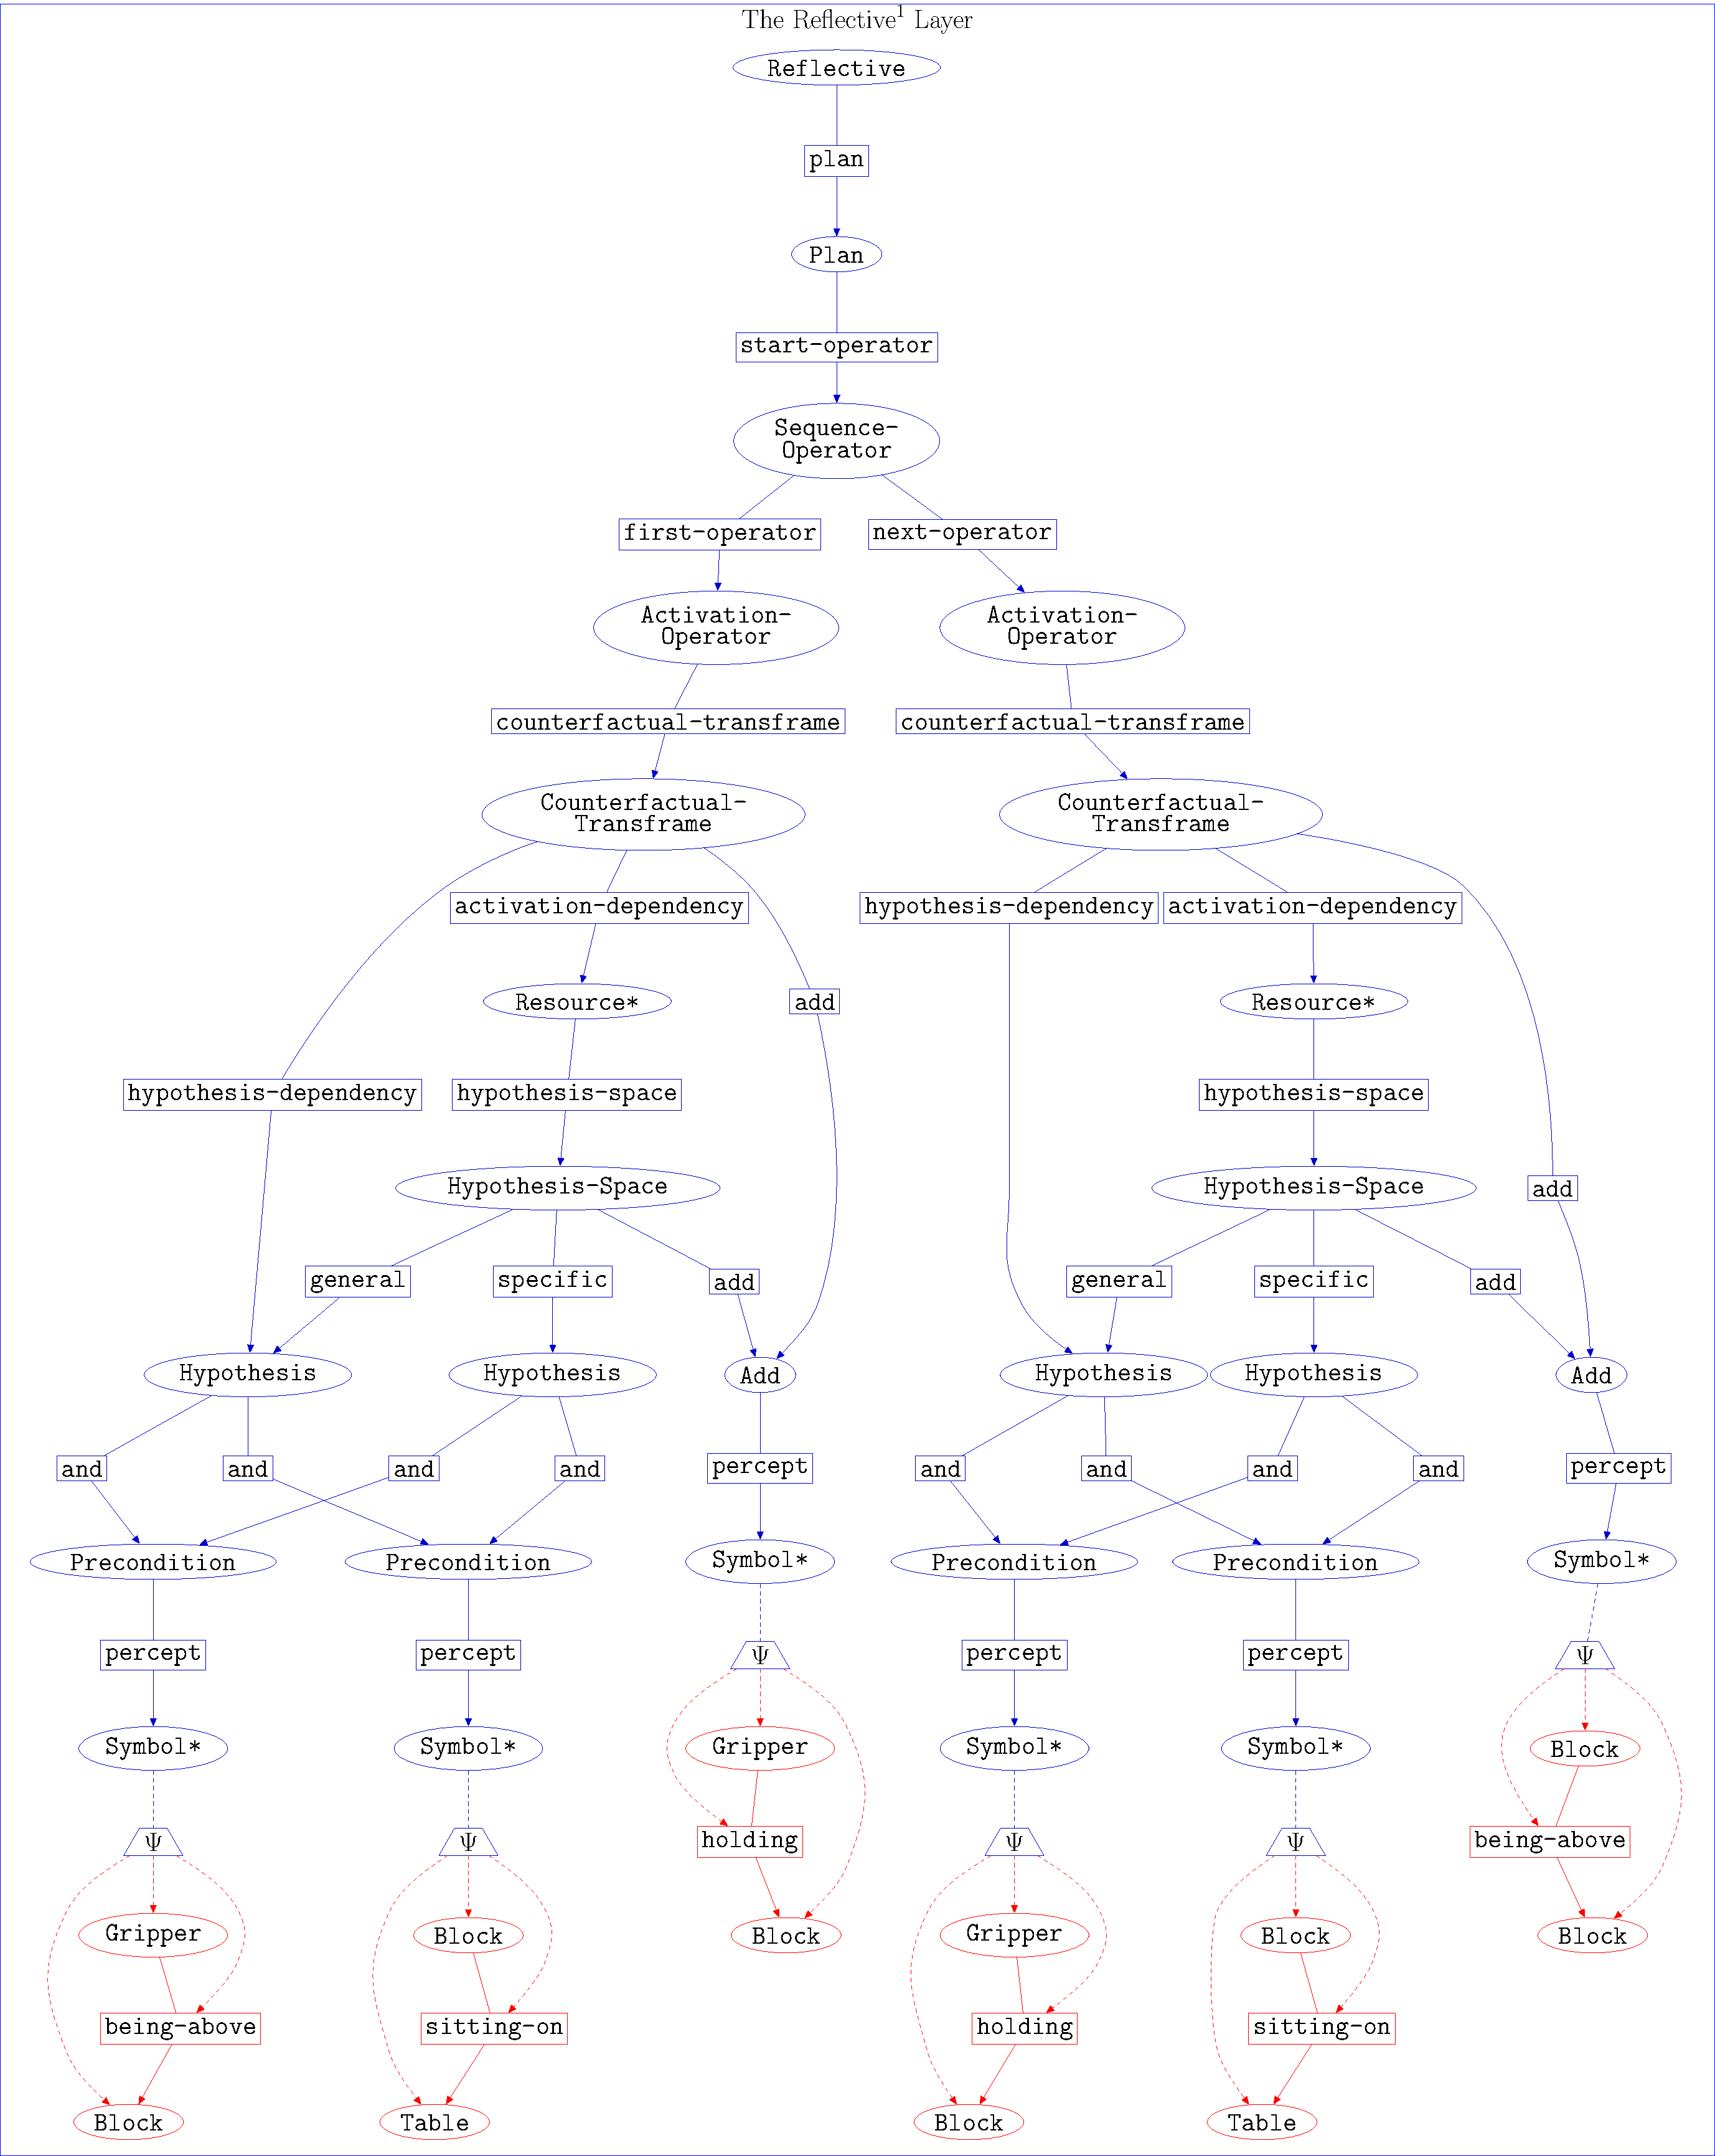
\includegraphics[width=18cm]{gfx/example_plan}
\caption[An example of a two-step plan.]{An example of a two-step
  plan.}
\label{figure:example_plan}
\end{figure}

\section{A Planning Machine}

The first-order reflective thinking layer makes plans in order to make
plans that will accomplish symbolic physical goals when executed.
{\mbox{\autoref{figure:example_planner}}} shows an example of a
planning machine.  In the model, a planning machine is a simple
computational machine with different registers that creates and
manipulates plan objects.  The operations of a first-order planning
machine can be seen as symbolic resources in the second-order
reflective thinking layer.  In general, planning operations can be any
kind of dynamic activity of the first-order reflective thinking layer.
Because the model is not yet advanced enough to abstract objects and
their subjective perspectives, this planning machine the resources in
the second-order reflective layer resemble the simple symbolic actions
of a RISC processor, which are like the symbolic bytecodes of a
virtual machine.  The simplest symbolic resources in the second-order
reflective layer are the following list of actions that simply move
plans between the different registers of the planning machine:
\begin{itemize}
\item {\tt focus-on-register-a*}: Copy the plan in {\tt register-a} to
  the {\tt focus} register.
\item {\tt focus-on-register-b*}: Copy the plan in {\tt register-b} to
  the {\tt focus} register.
\item {\tt focus-on-execution*}: Copy the plan in the {\tt execute}
  register to the {\tt focus} register.
\item {\tt copy-focus-to-register-a*}: Copy the plan in the {\tt
  focus} register to register {\tt a}.
\item {\tt copy-focus-to-register-b*}: Copy the plan in the {\tt
  focus} register to register {\tt b}.
\item {\tt execute-plan-in-focus*}: Copy the plan in the {\tt focus}
  register to the {\tt execute} register.
\item {\tt execute-plan-in-focus*}: Copy the plan in the {\tt focus}
  register to the {\tt execute} register.
\item {\tt stop-execution*}: Remove any plan from the {\tt execute}
  register.
\end{itemize}
\begin{figure}
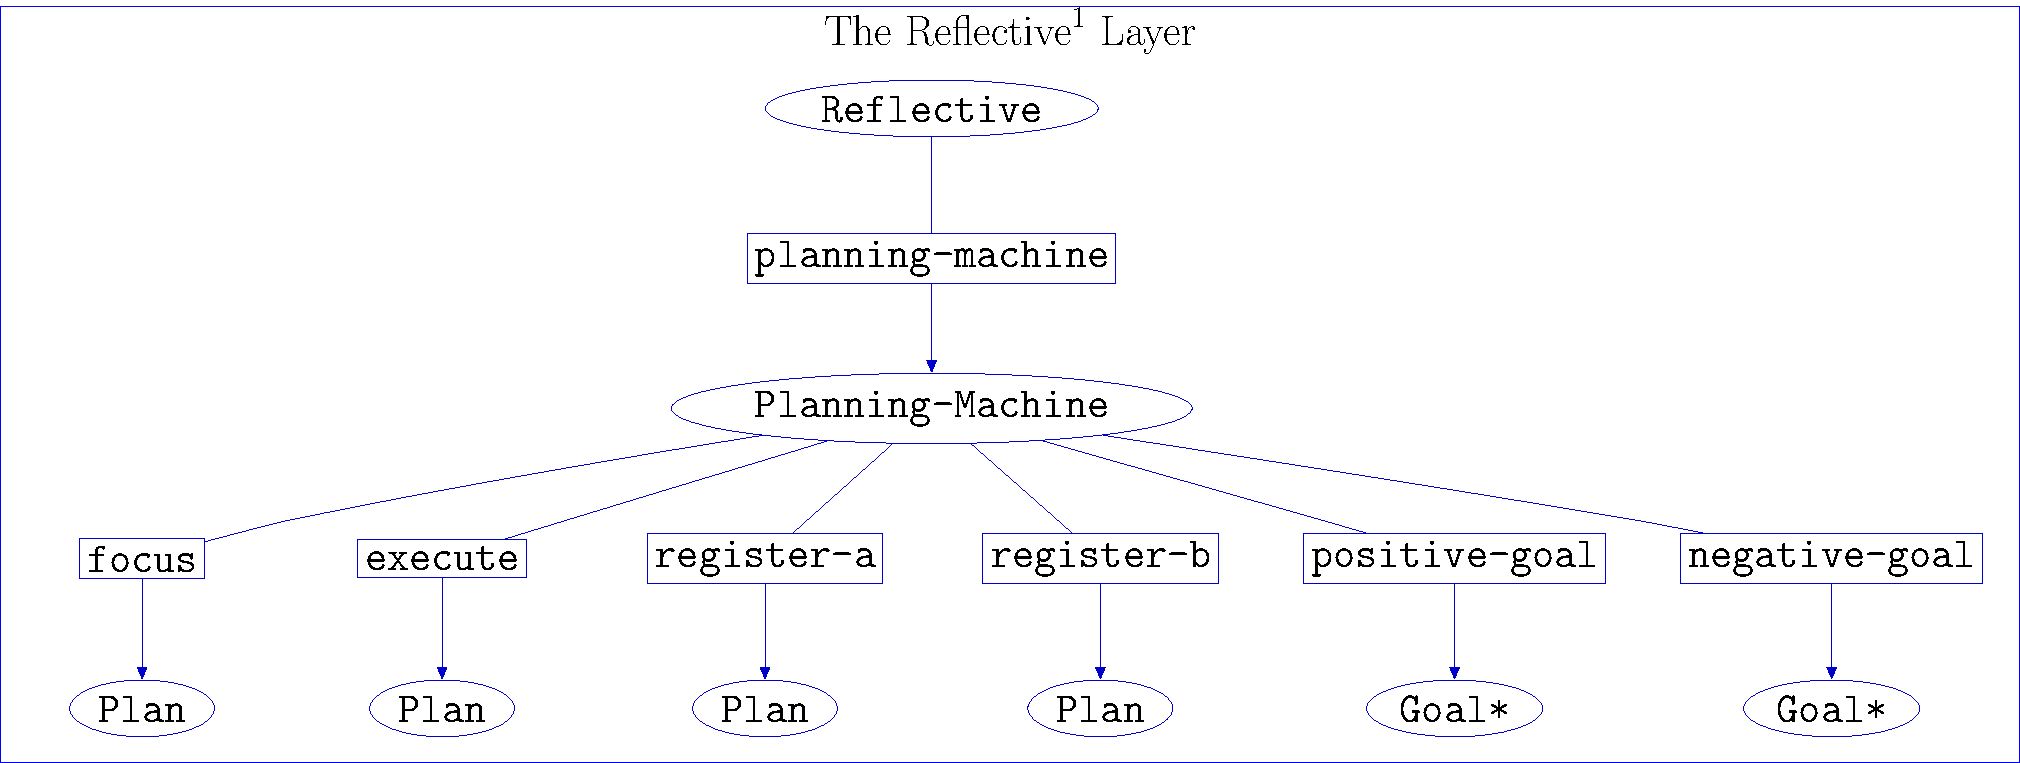
\includegraphics[width=12cm]{gfx/example_planner}
\caption[An example of a planning machine.]{An example of a planning
  machine.}
\label{figure:example_planner}
\end{figure}
The planning machine's execution register is a special register that
holds the plan that is currently executing.  As the planning machine
is like a virtual machine, plans are like computer programs for this
virtual machine.  The planning machine has a number of activities that
create plans that accomplish or avoid the current goals in the {\tt
  positive-goal} and {\tt negative-goal} slots of the planning
machine.  These activities are seen as symbolic resources that can be
used to accomplish planning goals by the second-order reflective
thinking layer.  Some of these plan creation and manipulation
resources in the second-order reflective thinking layer are as
follows:
\begin{itemize}
\item {\tt create-empty-plan*}: Create new plan with no operators and
  place in the {\tt focus} register.
\item {\tt extend-plan-greedy*}: Create new plan in the {\tt focus}
  register by adding a resource activation operator to the end of a
  duplicate of the plan in {\tt register-a}.  The new activation
  operator is chosen using a greedy technique that compares the
  options with a heuristic.
\item {\tt sequence-plans*}: Create new plan in the {\tt focus}
  register with a sequential program operator that orders a duplicate
  of the plan in {\tt register-a} as the {\tt first-operator} and a
  duplicate of the plan in {\tt register-b} as the {\tt
    next-operator}.
\item {\tt parallelize-plans*}: Create new plan in the {\tt focus}
  register with a parallel program operator that contains duplicates
  of the plans in {\tt register-a} and {\tt register-b}.
\item {\tt reverse-sequence*}: Create new plan in the {\tt focus}
  register with the reverse of a sequence operator in the plan in {\tt
    register-a}.  \cite{sussman:1973} mentions a related planning bug
  where preconditions of one action clobbers the preconditions of
  another, where the solution is sometimes simply reversing the
  actions in the plan.
\item {\tt parallelize-sequence*}: Create new plan in the {\tt focus}
  register replacing a parallel program operator with a sequence
  operator in the plan in {\tt register-a}.
\end{itemize}
These first-order reflective planning operators can be used by the
second-order reflective layer in order to make second-order plans that
control the first-order planning machine.

\section{Symbolizing Goals}

Positive and negative first-order planning machine goals are
symbolized from the $\text{reflective}^0$ layer of physical activity.
Note the bottom-up type of goal-oriented control in the model.  Also,
because reflective thinking layers are thought of as running
concurrently in the model, there is no necessary priority for devoting
thinking resources to any specific layer of thinking as more important
than another.  The implementation includes built-in goals that have
already been symbolized as positive goals that are included as part of
the first-order reflective planning machine.

\section{Second-order Resources}

The second-order reflective layer is the lowest layer that is able to
symbolize references to the dynamic activities of reflective thinking.
Although not included in the implementation, here is a list of
examples of symbolic resources that could exist in the reflective
thinking layers of order two or greater:
\begin{itemize}
\item {\tt complete-execution*}: Copy the plan in the {\tt focus}
  register to the {\tt execute} register and wait for the plan to
  complete execution, resulting in either failures or success.
\item {\tt refine-symbolic-perception*}: Create a new symbol that
  divides the currently perceived symbols into smaller subgraphs of
  dynamic activity that may be helpful for accomplishing or avoiding
  the positive and negative goals currently in the planning machine.
\item {\tt refine-symbolic-resource*}: Create a new symbol that refers
  to a subgraph of the current symbolic resource references.
\item {\tt create-type-perception*}: Create a new symbol that refers
  to the logical ``or'' or disjoint perception of two or more symbolic
  perceptual references.
\item {\tt create-analogical-plan*}: Create a new plan in the {\tt
  focus} register that satisfies the \cite{winston:1970}
  difference-of-differences relationship between the plans in {\tt
    register-a} and {\tt register-b} when applied to {\tt register-c}.
  This algorithm has been implemented by Panupong Pasupat and is
  included in the ``analogy'' package of the implementation, but is
  not included in my proof of concept demonstrative example.
\end{itemize}

\section{Critical Failure Heuristics}

\cite{sussman:1973} introduced the idea of a critical planning
heuristic, which is based upon a logical search and pattern
recognition algorithm.  Building on this work, \cite{singh:2003,
  singh:2005a} describe a variety of critical first-order and
second-order reflective resources, many of which assume a logical
search over an object oriented social model.  I have taken painstaking
efforts to not introduce any logical problem solving into my
algorithm, so that each basic step in my planning machine that compose
more complex planning actions takes a predictable constant time
complexity, $O(1)$.  This allows all critical and logical search
algorithms in my model to be implemented in a way that is reflected
upon and optimized by the critical learning algorithm itself.
\cite{minsky:2006} describes a ``critic-selector'' algorithm as
follows:
\begin{quote}
Each Critic ... can recognize a certain species of ``Problem Type.''
When a Critic sees enough evidence that you now are facing its type of
problem, then that Critic will activate what we shall call a
``Selector,'' which tries to start up a set of resources that it has
learned is likely to act as a Way to Think that may help in this
situation.
\end{quote}
I use critics in my model to predict different types of reflective
plan execution failures.

\section{Planning Failures}

Planning may fail in a number of different ways in a reflective
layered system.  Note that while planning may fail, the
$\text{reflective}^0$ physical layer of activity does not include the
concept of failure because this layer contains neither symbolic
perceptions, actions, nor goals.  The physical layer is the given,
goals are symbolized in the first-order reflective layer, so this
layer of activity is the first layer that may fail to accomplish its
own created goals.

The most common type of failure that is discussed in the literature is
an expectation failure.  This is the type of failure that I
demonstrate in the implementation.  \cite{cox:2007a} discusses a
number of different self-reflective failures in story understanding
that are based on a logical search algorithm.  My model is more basic
than most approaches to implementing artificial reflective thinking
because it carefully avoids any logical resolution search algorithm
that operates behind the scenes.  Although, this model does not have a
predefined object-oriented (or subject-oriented) view of problem
solving, there are still a variety of interesting types of plan
failure that occur at this level of reflective debugging.  I have
discussed two types of first-order plan execution failures, here
listed as critical failures followed by a selective response:
\begin{itemize}
\item {\tt expectation-failure} $\longrightarrow$ \\
      {\tt refine-resource-transframe-hypotheses}
\item {\tt activation-conflict-failure} $\longrightarrow$ \\
      {\tt create-parallel-suppression-plan}
\item {\tt failure-to-distinguish-predictions} $\longrightarrow$ \\
      {\tt refine-symbolic-perceptions-and-resources}
\item {\tt exhausted-hypothesis-space} $\longrightarrow$ \\
      {\tt generalize-hypothesis-language}
\item {\tt activation-failure} $\longrightarrow$ \\
      {\tt create-new-symbolic-resources}
\end{itemize}

\section{Factual Plan Failure Knowledge}

When the planning machine executes a plan, the plan may encounter a
bug, a failure.  Failed plans, failed counterfactual knowledge, and
their untrue hypothesis dependencies are not immediately discarded in
a reflective learning algorithm as is the case with non-reflective
learning algorithms.  These failure events are factual knowledge about
the actual use of counterfactual knowledge.  Factual failure knowledge
is used to learn hypothetical knowledge about what plan structures in
the context of current physical perceptions are prone to specific
types of failure.  Given a factual plan failure event, different
symbolic types of failure can be predicted from given plan structures
in the context of the layers below the planning machine.
{\mbox{\autoref{figure:example_plan_failure}}} shows an example of a
one-step plan with a factual expectation failure structure.
\begin{figure}
\hspace*{-3cm}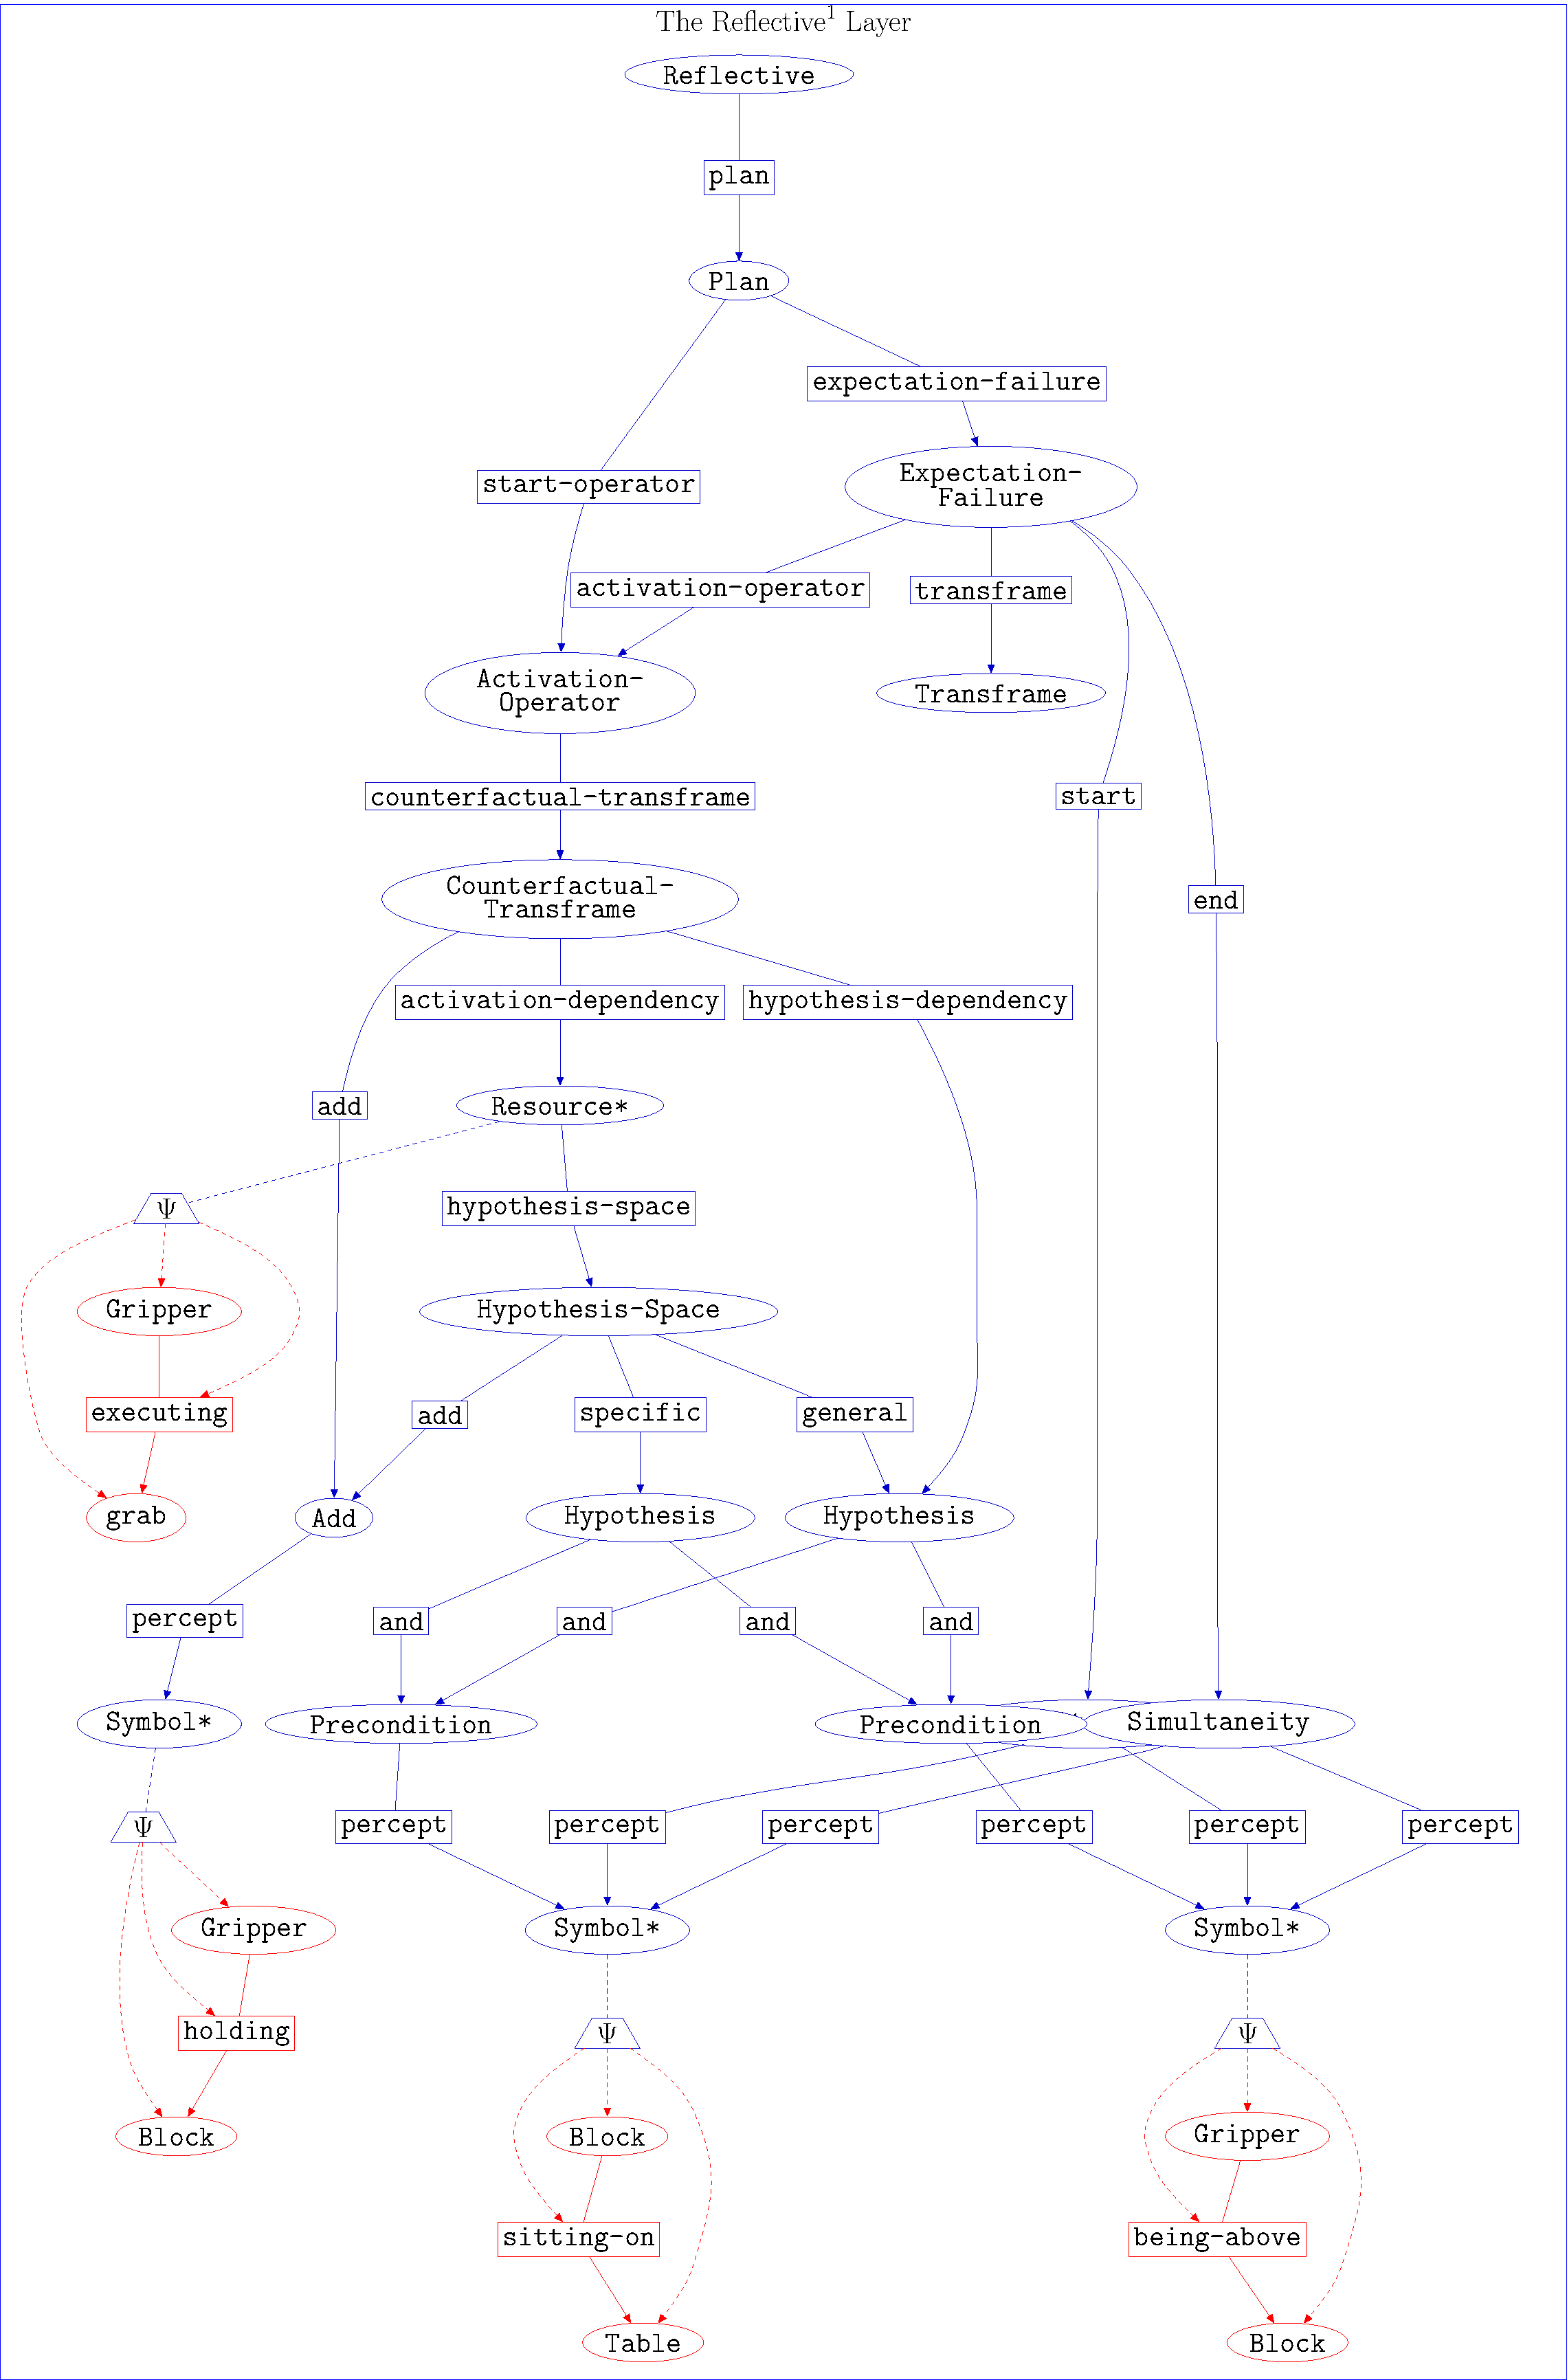
\includegraphics[width=16cm]{gfx/example_plan_failure}
\caption[An example of a one-step plan with a factual expectation
  failure.]{An example of a one-step plan with a factual expectation
  failure, where the gripper is expected to pick up the block, but the
  factual transframe shows that nothing actually happens in this case
  of execution.  This could be due, for example, to the block being
  glued to the table or some other unconsidered hypothesis.}
\label{figure:example_plan_failure}
\end{figure}

\section{Prediction of Failure Based on Plan Structure}

The second-order reflective thinking layer creates symbolic references
to both the first-order reflective thinking layer as well as the
physical layer of activities.  Resources in the second-order
reflective thinking layer control the activities in layers below,
including the planning machine's manipulation of plan structures.
Second-order hypothesis spaces are learned in order to predict the
transitional effects of first-order reflective planning machine
activities.  The second-order hypothesis spaces contain hypothetical
knowledge about the actual factual use of counterfactual knowledge.
While goals in the second-order reflective thinking layer can be
specifically about physical activities, the power of second-order
reflective goals comes from considering goals that are abstracted from
this physical layer of activity.  For example, a second-order
reflective thinking goal could be to control the planning machine in
order to work against the first-order goals.  The first-order planning
machine activities can be thought of as plans being executed by the
second-order planning machine.
{\mbox{\autoref{figure:example_critical_failure_heuristic}}} shows an
example of planning machine symbolic perceptions.
\begin{figure}
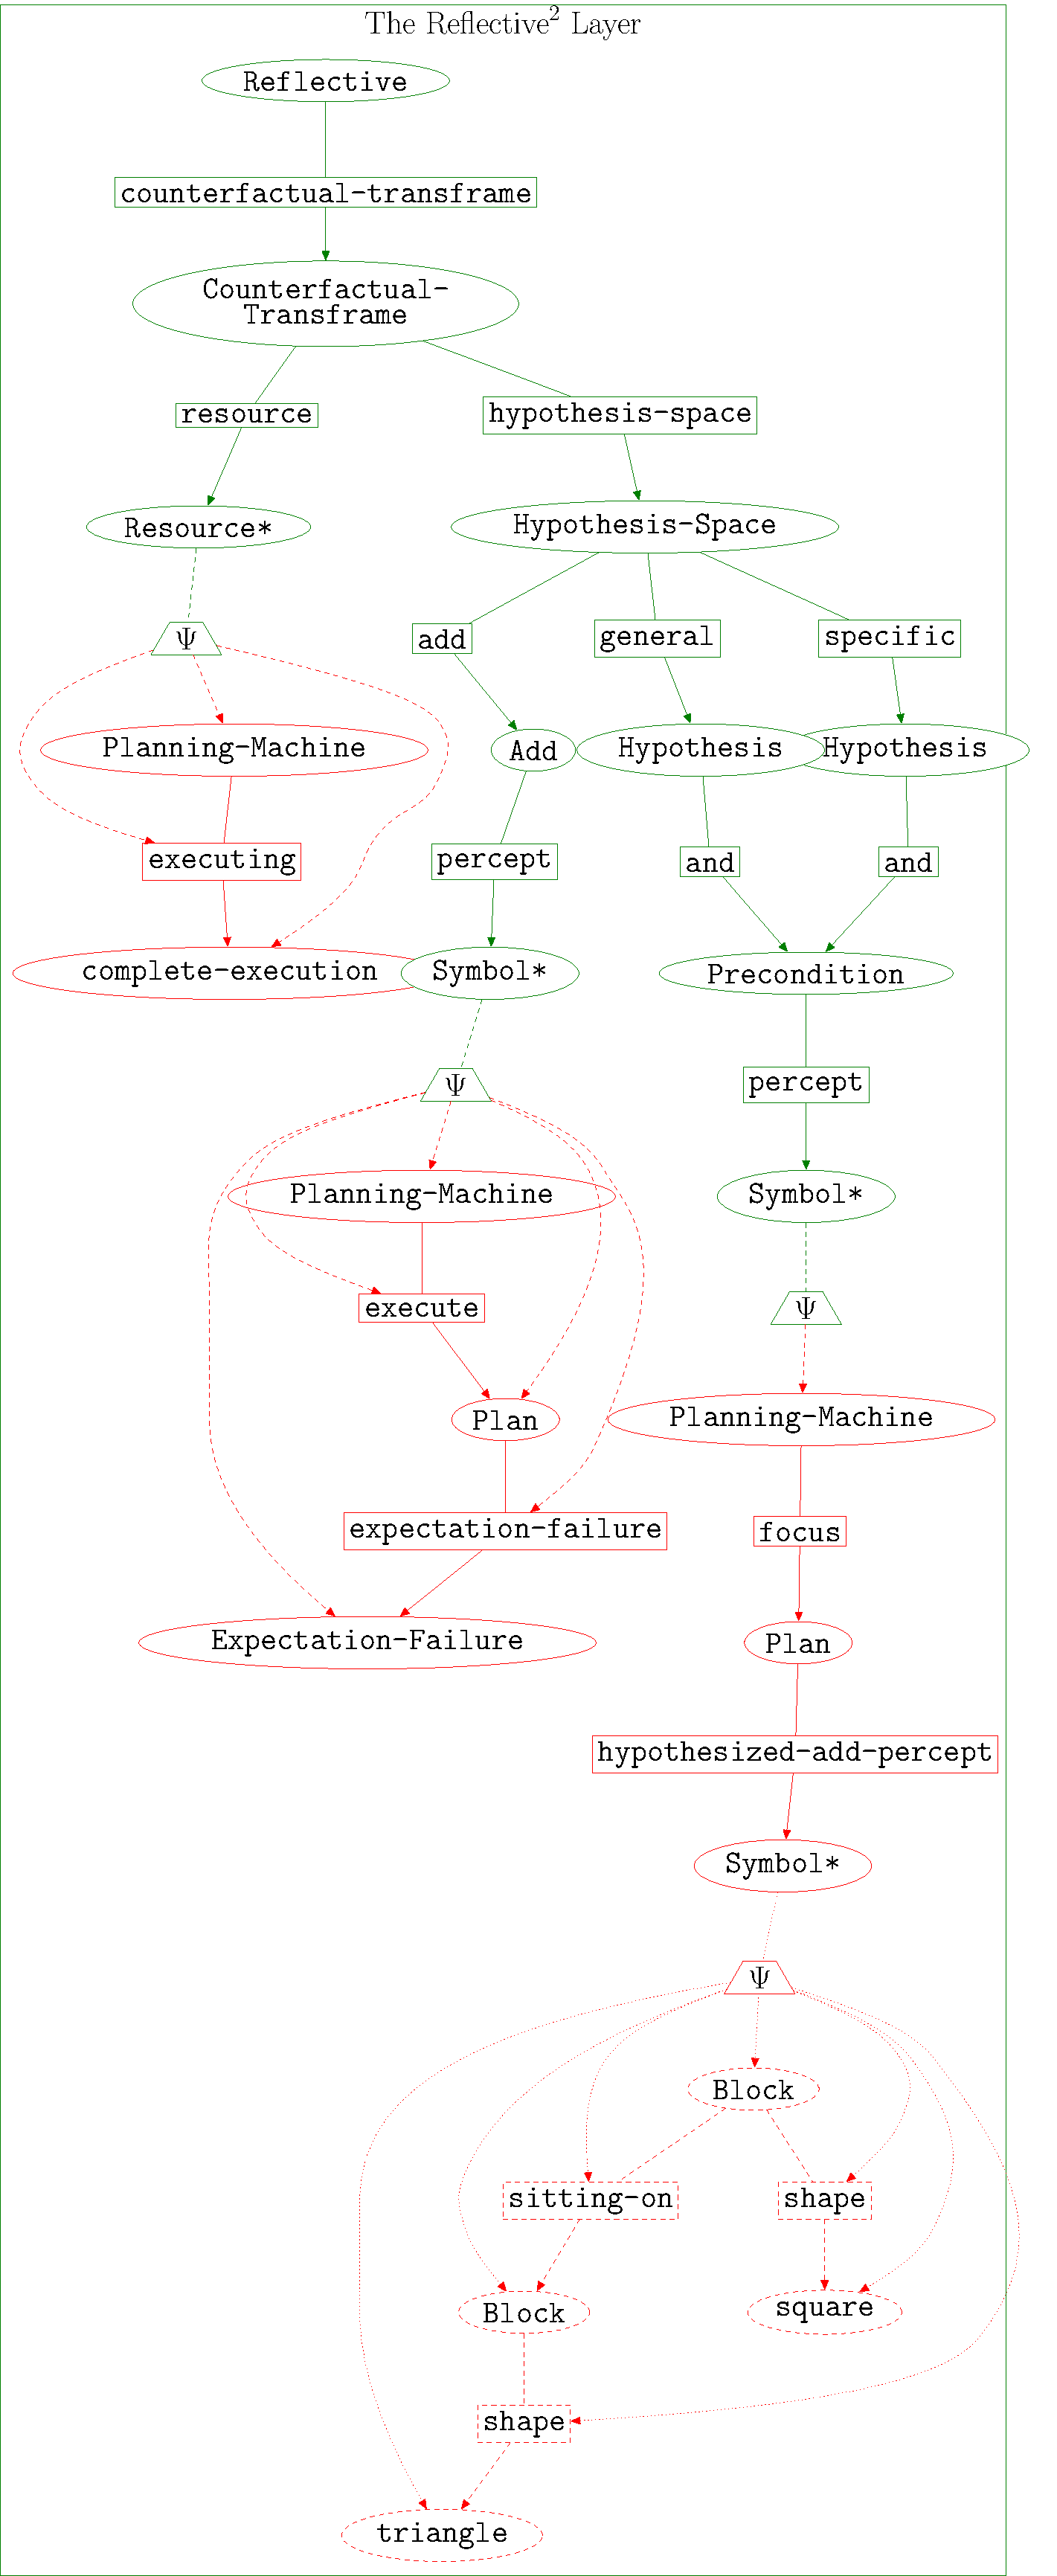
\includegraphics[width=10cm]{gfx/example_critical_failure_heuristic}
\caption[An example of a second-order counterfactual transframe
  predicting a plan execution failure.]{An example of a second-order
  counterfactual transframe predicting a plan execution failure.  In
  this example, a plan that hypothesizes the creation of a stack of
  blocks with a square block stacked on top of a triangle block is
  predicted to lead to an expectation failure if it were to be
  executed.}
\label{figure:example_critical_failure_heuristic}
\end{figure}

